\documentclass[12pt]{article}

% Packages:
\usepackage{graphicx}
\usepackage[portuguese]{babel}
\usepackage[utf8]{inputenc}
\usepackage{setspace}
\usepackage{listings}
\usepackage{hyperref}
\usepackage{tocloft}
\usepackage{fancyhdr}
\usepackage{placeins}
\usepackage{subcaption}
\usepackage{subfiles}
\usepackage{outlines}
\usepackage{indentfirst}
\usepackage{amsmath}
\usepackage{enumerate}
\usepackage{subfiles}
\usepackage{color, colortbl, xcolor}
\usepackage{multicol}
%---

% Options:
\setstretch{1} % Espaçamento entre linhas
\usepackage[top=3cm, bottom=2cm, left=1.5cm, right=1.5cm]{geometry}
\PassOptionsToPackage{hyphens}{url}
\title{}
\date{}

% Code customization:
% Default fixed font does not support bold face
\DeclareFixedFont{\ttb}{T1}{txtt}{bx}{n}{10} % for bold
\DeclareFixedFont{\ttm}{T1}{txtt}{m}{n}{10}  % for normal

\lstset{
	basicstyle=\footnotesize,
	columns=fullflexible,
    keywordstyle=\ttb\color{blue},
	stringstyle=\ttm\color{green},
	commentstyle=\color{gray},
	frame=None,
	breaklines=true,
	showstringspaces=false,
	postbreak=\mbox{\textcolor{red}{$\hookrightarrow$}\space},
}

%---
% Document:
\begin{document}
	% Cabeçalho:
\begin{figure}
		\begin{minipage}{.3\linewidth}
			\centering
			
\includegraphics[width=.6\linewidth]{imgs/ufpa.jpg}
		\end{minipage}
		\begin{minipage}{.70\linewidth}
			\flushleft
			\paragraph{}
			\textbf{ }\newline
			\textbf{UNIVERSIDADE FEDERAL DO PARÁ} \newline
			\textbf{INSTITUTO DE TECNOLOGIA} \newline
			\textbf{FACULDADE DE ENGENHARIA DA COMPUTAÇÃO E TELECOMUNICAÇÕES} \newline
			\textbf{TE05205 - Top. Especiais em Engenharia de Computação II} \newline
            \textbf{Prof. Dr. Roberto Celio Limão de Oliveira} \newline
            \textbf{Aluna: Camila Novaes Silva (201606840055)}
		\end{minipage}
\end{figure}
\FloatBarrier
\begin{center}
    {\Large \textbf{Exemplo 02 de Otimização - Função f6}}
\end{center}
%%%%%%%%%%%%%
\hfill

O Algoritmo genético (AG) descrito a seguir foi implementado para solucionar um exemplo
de otimização, especificamente o de maximização da função $f6$ de duas variáveis. A função a ser
maximizada é
$$f(x,y) = 0.5 - \frac{[\sin(\sqrt{(x^2 + y^2)})]^2 - 0.5}{[1 + 0.001(x^2 + y^2)]^2}$$.

% trim: left lower right upper
\begin{figure*}[htb]
	\begin{center}
	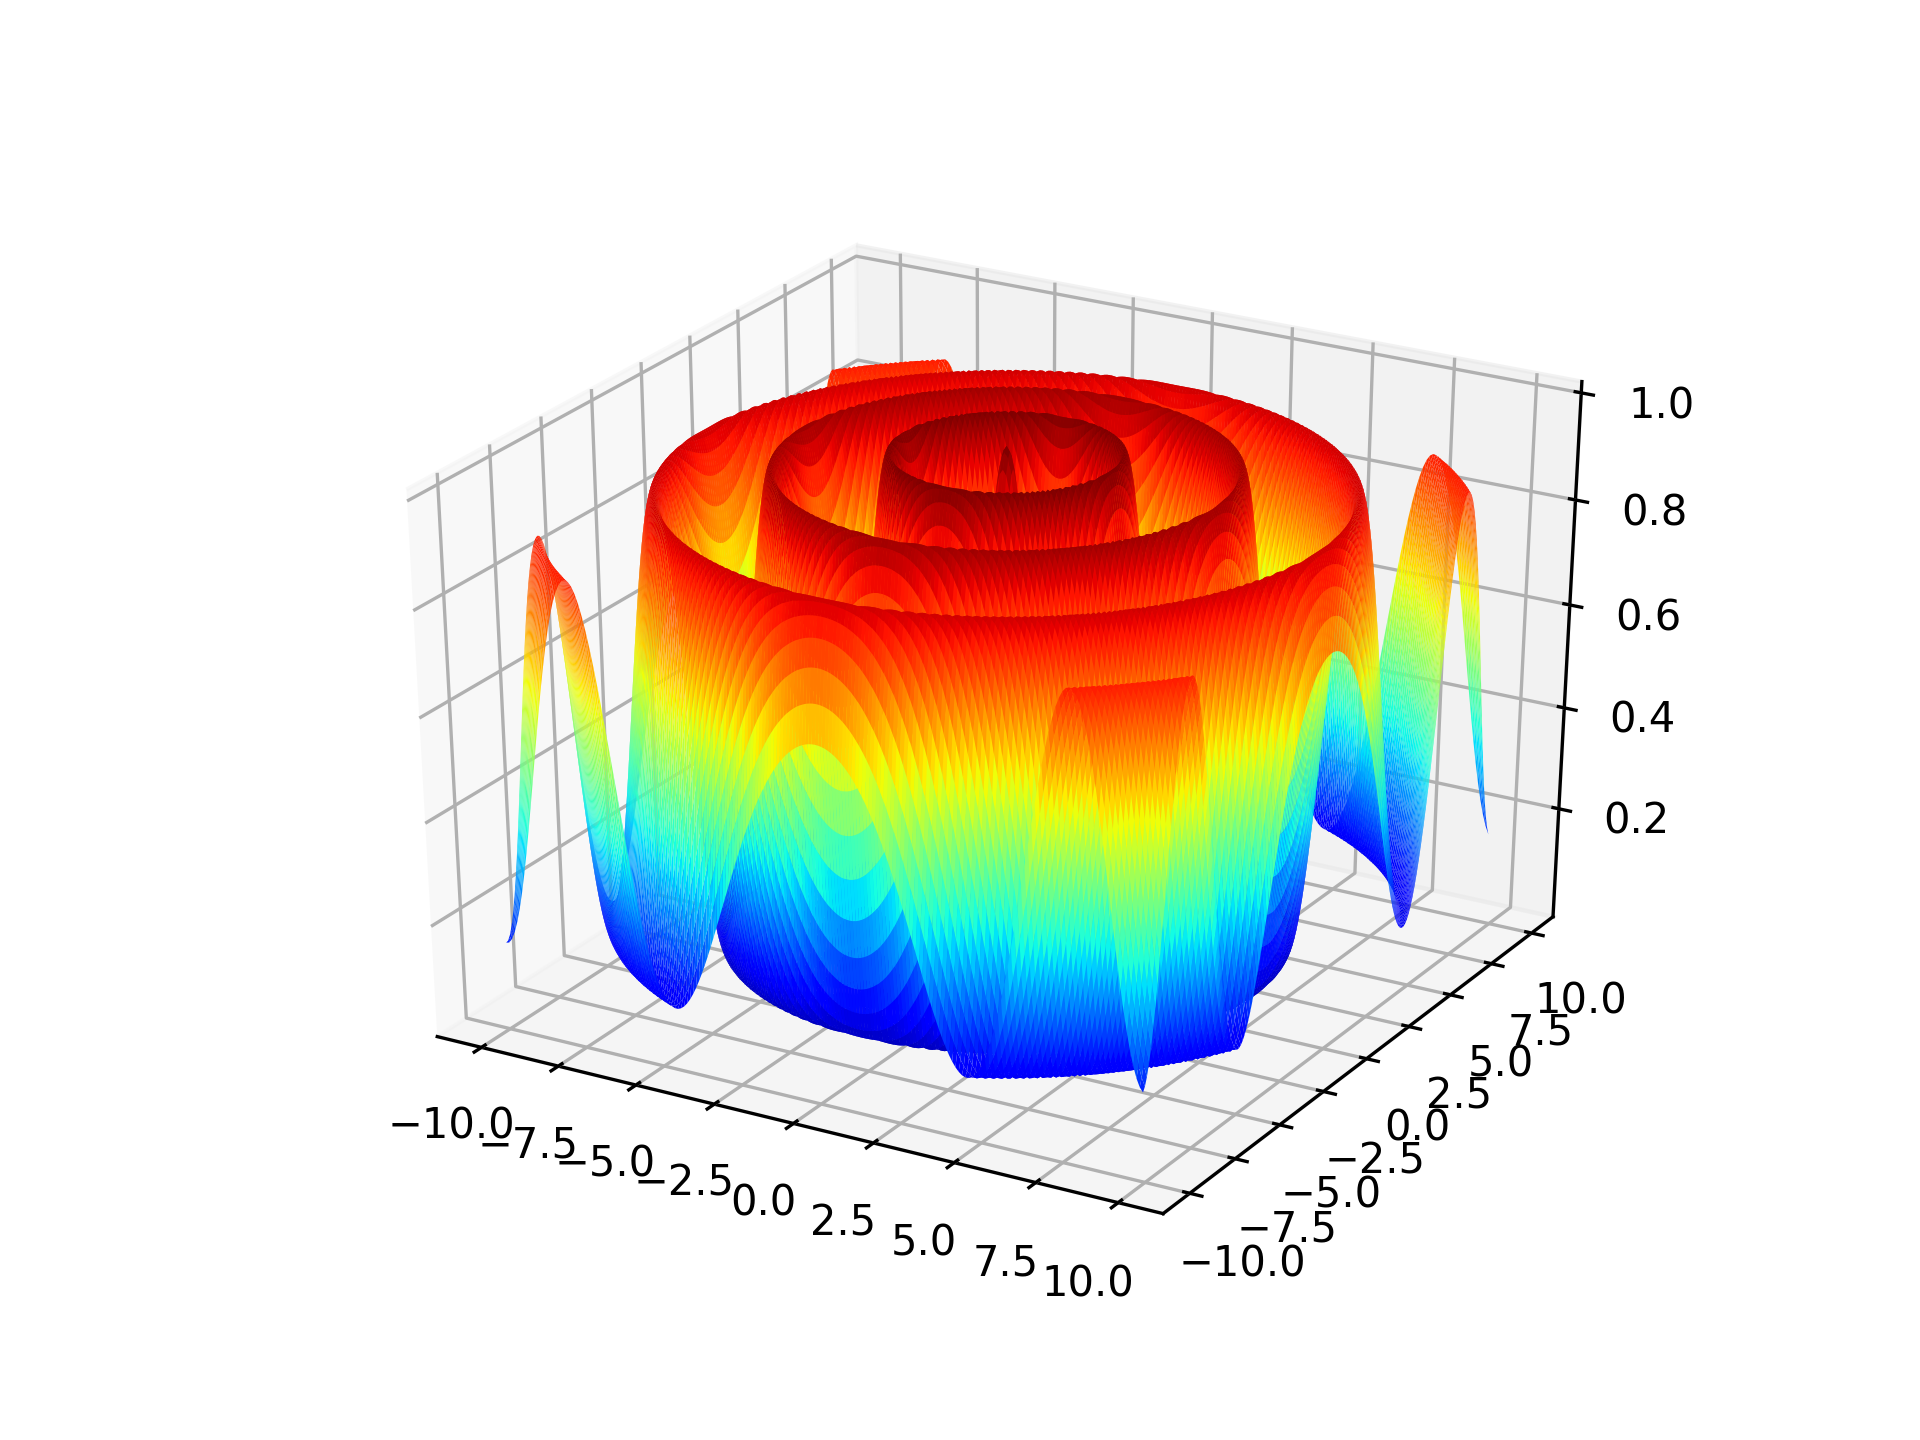
\includegraphics[trim={0.5cm 1cm 1cm 2cm},clip,width=0.5\textwidth]{./imgs/function.png}
	\caption{Função F6.\label{fig:result}}
	\end{center}
\end{figure*}

Assim, o objetivo é encontrar o valor de $x$,$y \in [-100,100]$ que maximiza a função $f$.

\begin{enumerate}[\textbf{(i)}]
	\item \textbf{Representação}
		\subitem Para representar todos os valores dentro do intervalo $[-100,100]$, com uma precisão
		de 5 casa decimais foram necessários 25 bits para cada variável,
		$$16777216 = 2^{24} < 200*10^5 \leq 2^{25} = 33554432$$
		\subitem Assim, para a decodificação entre real e binário foram utilizadas as seguintes equações:
		$$x_{real} = d(x') =  -100 + x' * \frac{200}{2^{25} - 1}$$
		$$y_{real} = d(y') =  -100 + y' * \frac{200}{2^{25} - 1}$$
		\subitem Onde $x'$ é a conversão direta da base binária para a decimal.

	\item \textbf{Seleção}
		\subitem Algoritmo de seleção utilizado foi a roleta proporcional ao fitness. Onde a função de
		avaliação é igual a $f(x,y)$.
	\item \textbf{Operadores genéticos}
		\subitem Para realizar o cruzamento, foi utilizado o algoritmo ponto de corte, com uma taxa de 
		cruzamento de 75\%. E para a mutação foi utilizada uma taxa igual a 1\%.
	\item \textbf{Critério de paragem}
		\subitem O critério de paragem foi 100 gerações.
\end{enumerate}

Os resultados obtidos são apresentados nas figuras abaixo.

\begin{figure}[htb]
		\centering
		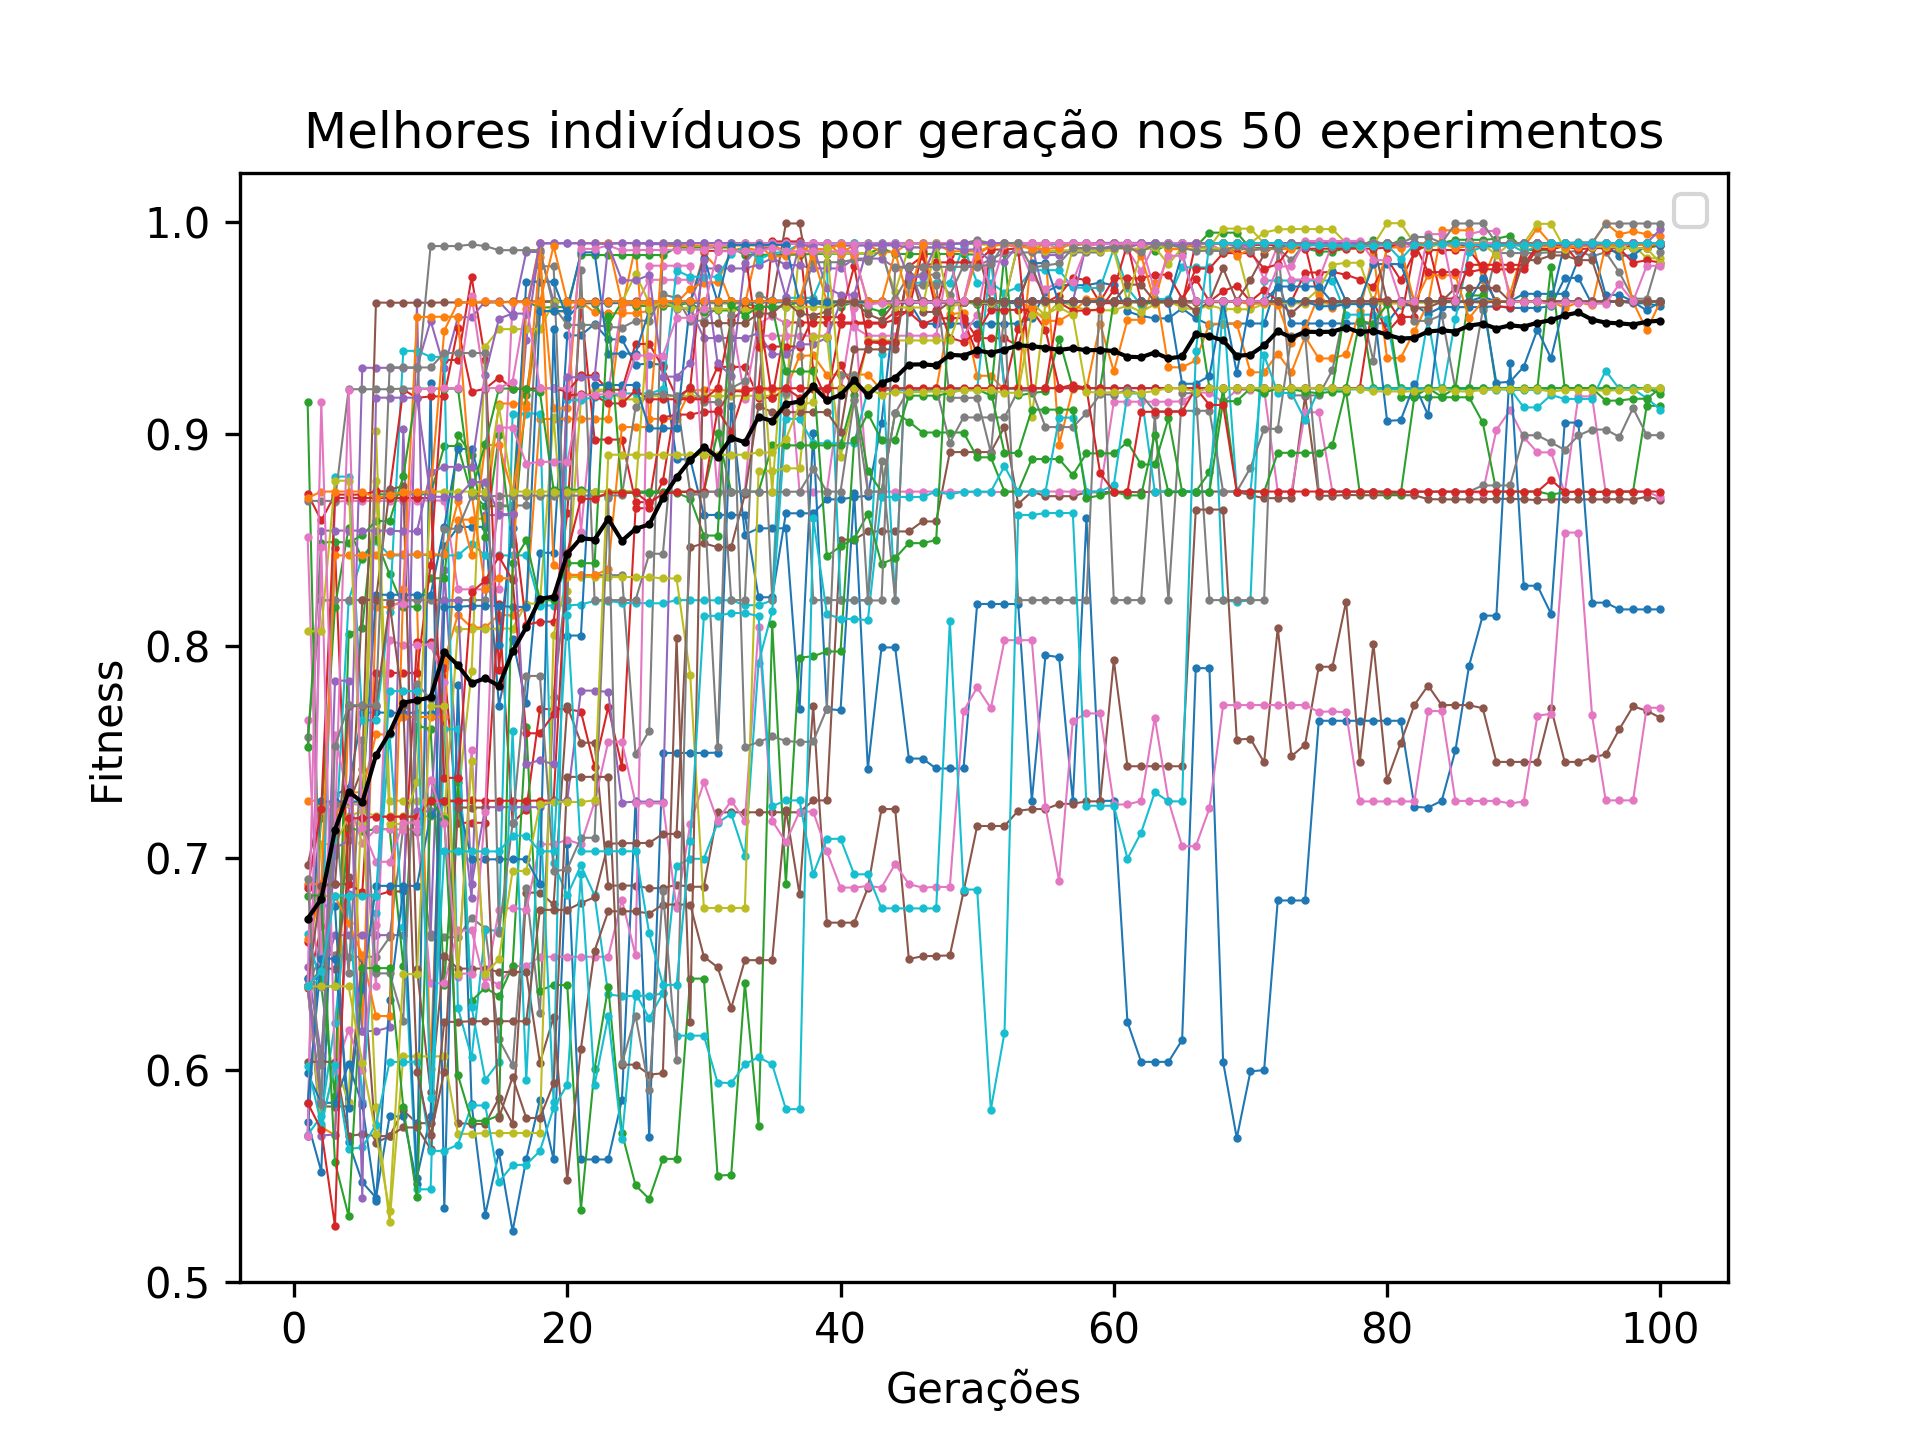
\includegraphics[width=0.9\textwidth]{./imgs/fitness_vs_exp_best.png}
		\caption{Melhores indíviduos de todos os experimentos ao longo das gerações.
		Em preto é mostrado o comportamento médio dos 50 experimentos.}
\end{figure}

\begin{figure}[htb]
	\centering
	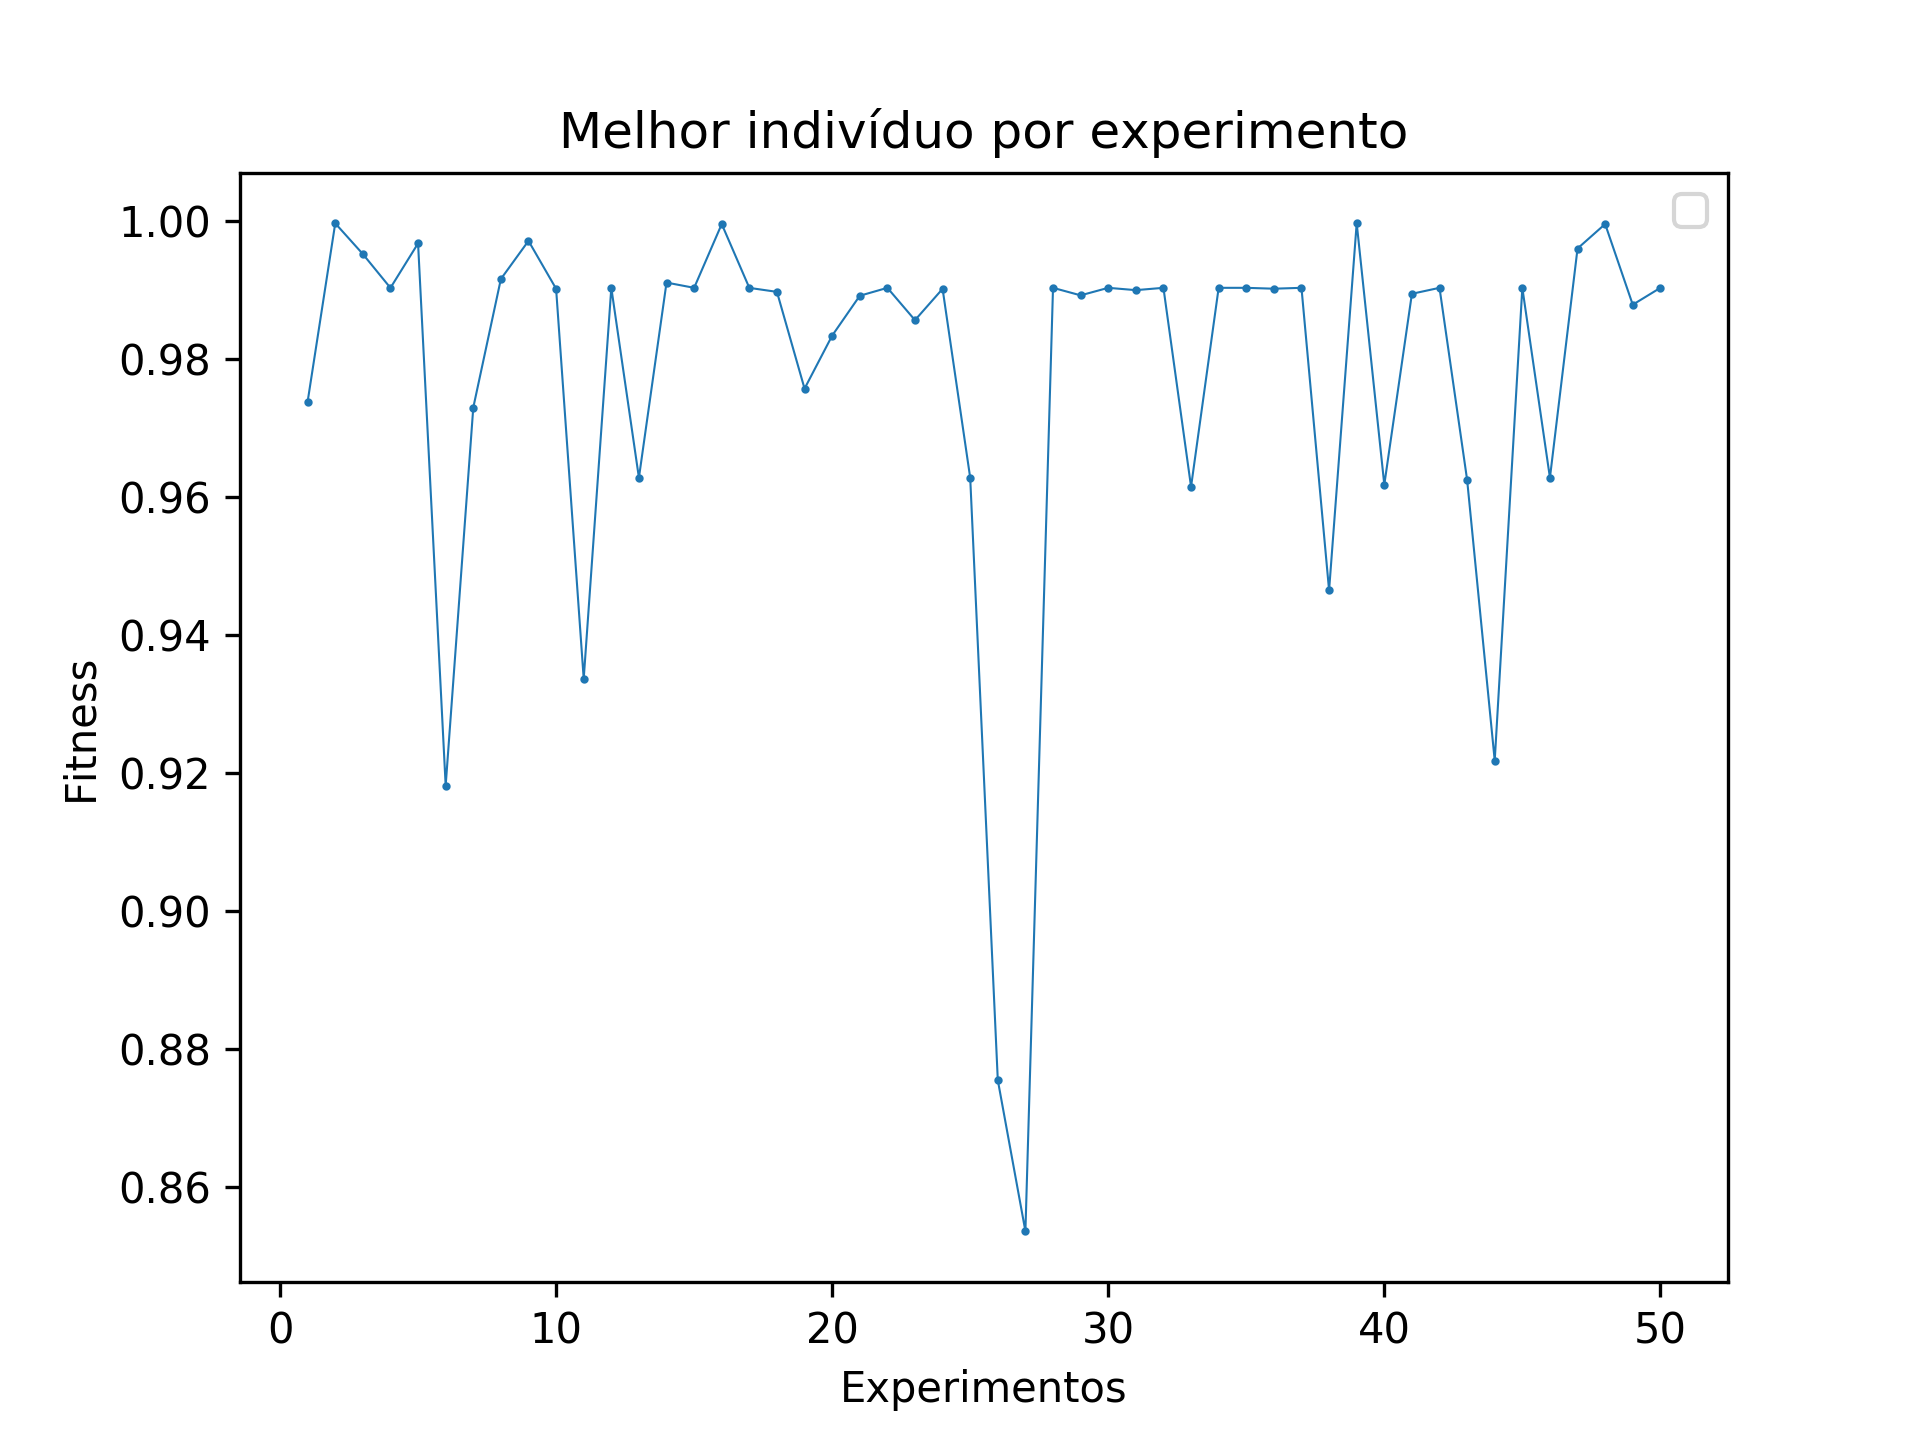
\includegraphics[width=0.9\textwidth]{./imgs/fitness_vs_best.png}
	\caption{Melhor indíviduo nos 50 experimentos.}
\end{figure}

\begin{figure}[htb]
	\centering
	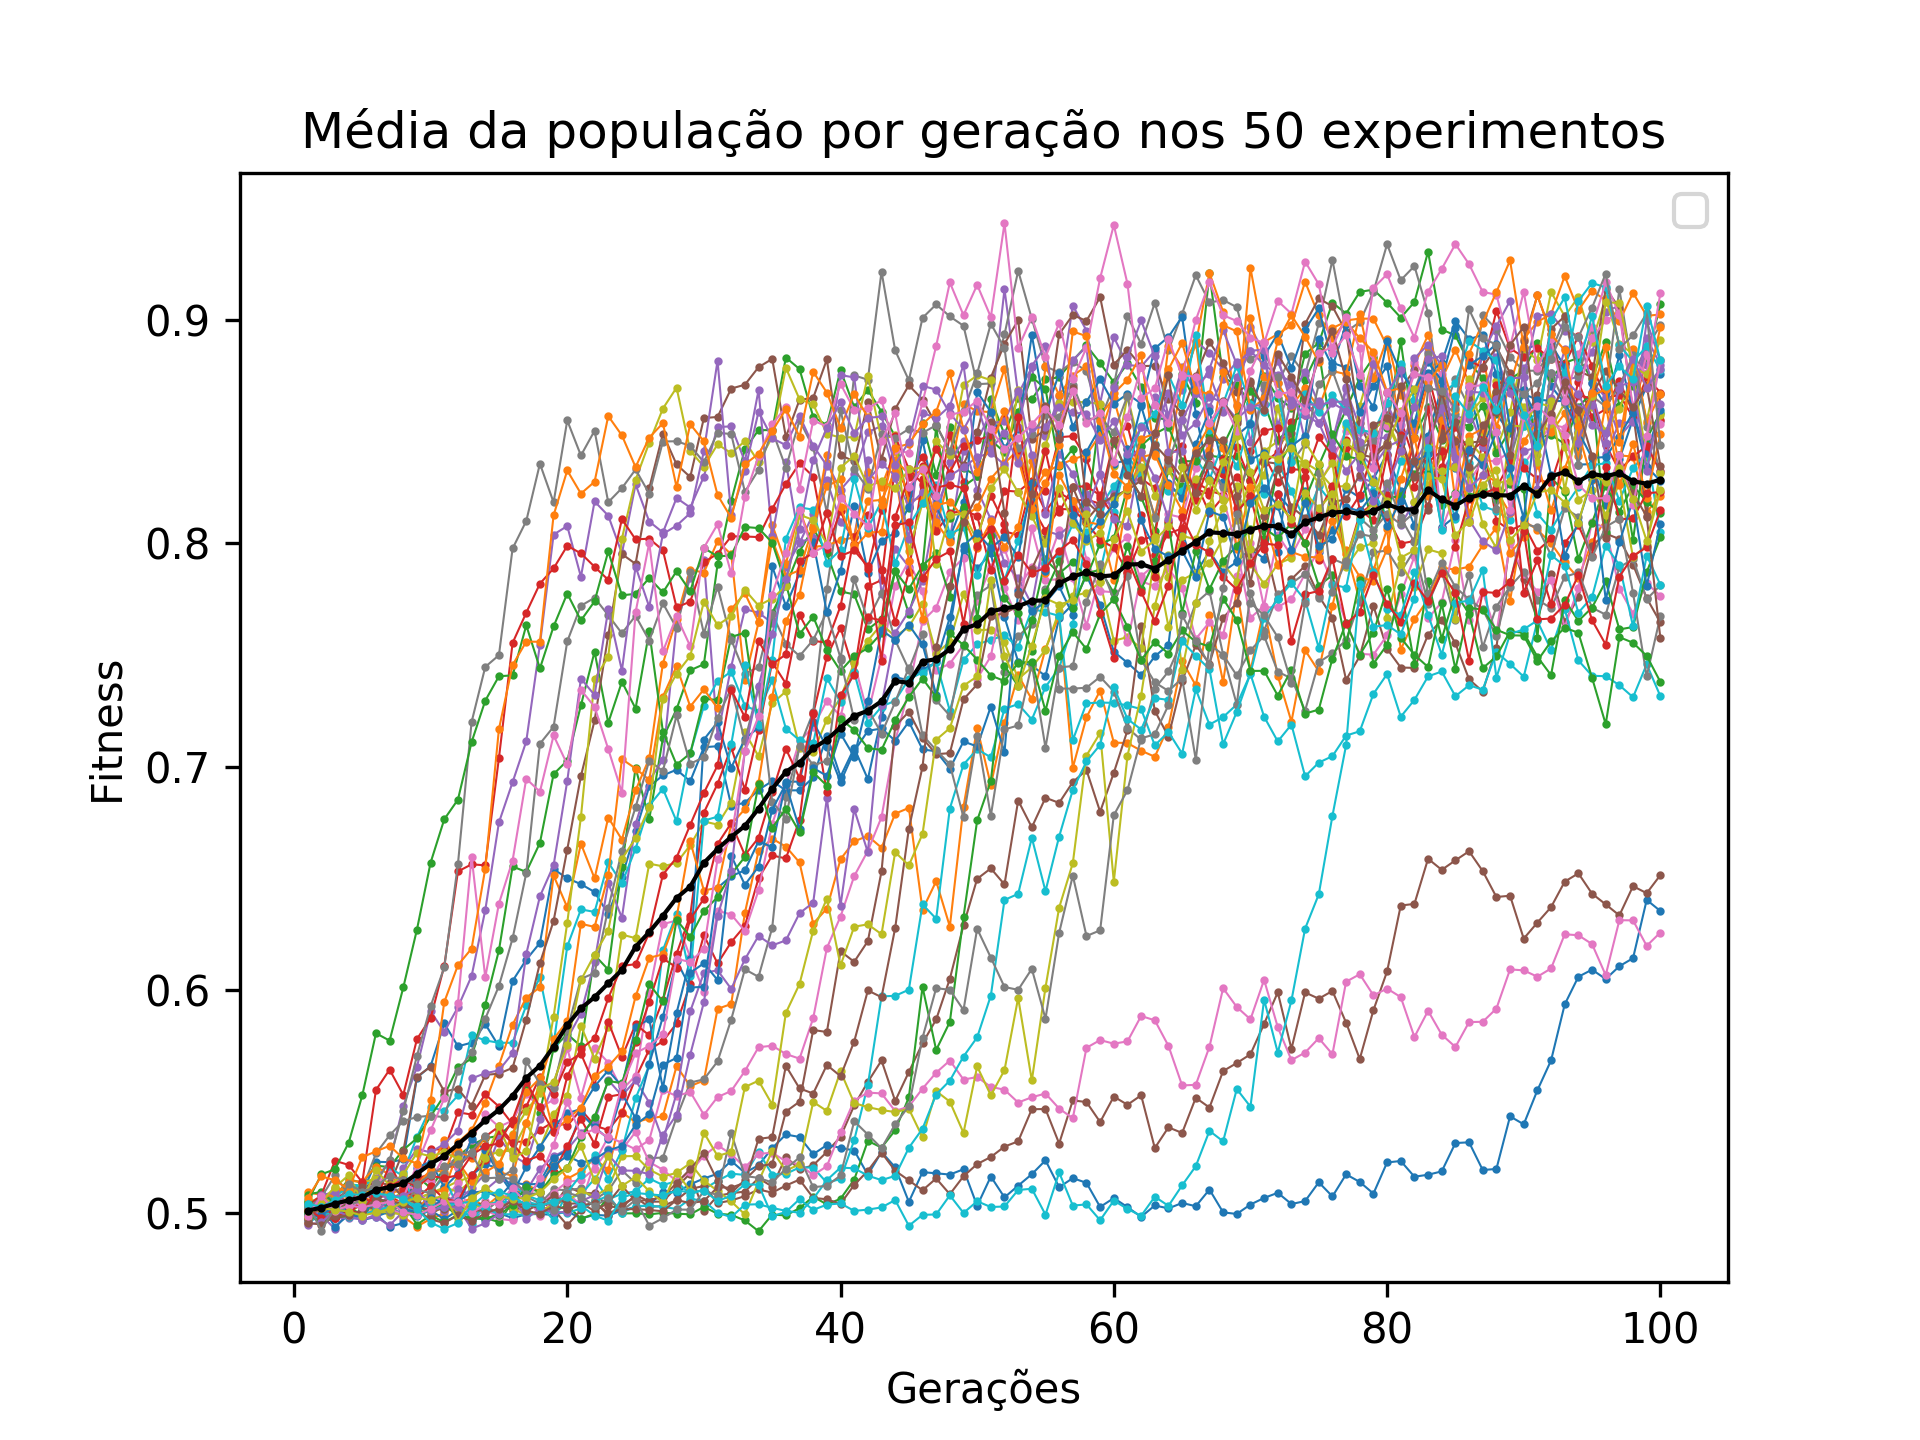
\includegraphics[width=0.9\textwidth]{./imgs/fitness_vs_exp_mean.png}
	\caption{Média da população de todos os experimentos ao longo das gerações.
	Em preto é mostrado o comportamento médio dos 50 experimentos.}
\end{figure}

\begin{figure}[htb]
	\centering
	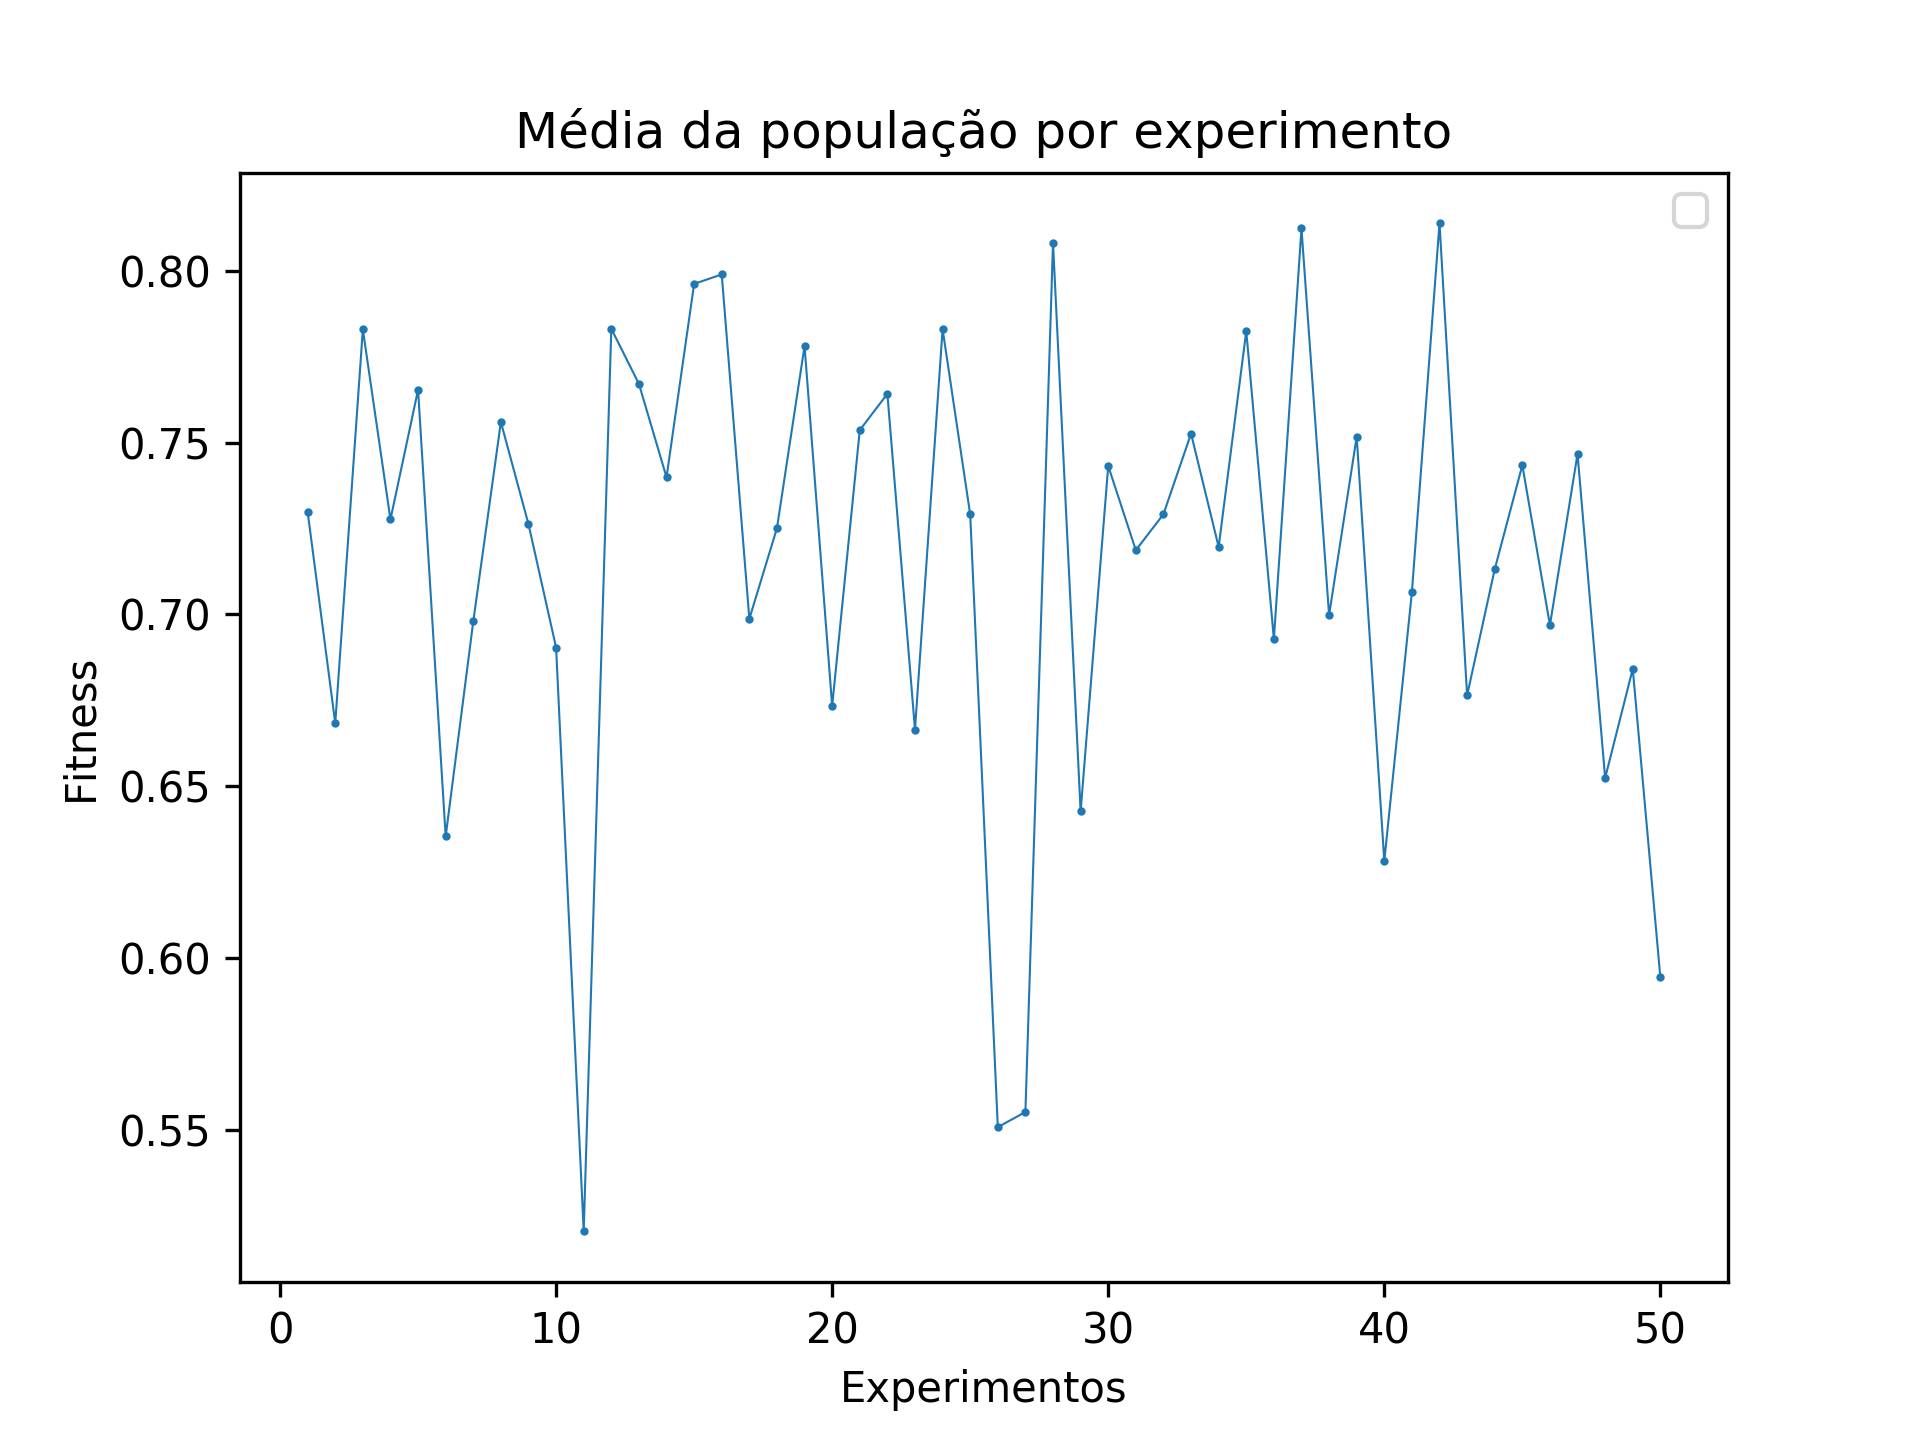
\includegraphics[width=0.9\textwidth]{./imgs/fitness_vs_mean.png}
	\caption{Média da população nos 50 experimentos.}
\end{figure}

	\begin{figure}[htb]
	\begin{subfigure}{.5\textwidth}
		\centering
		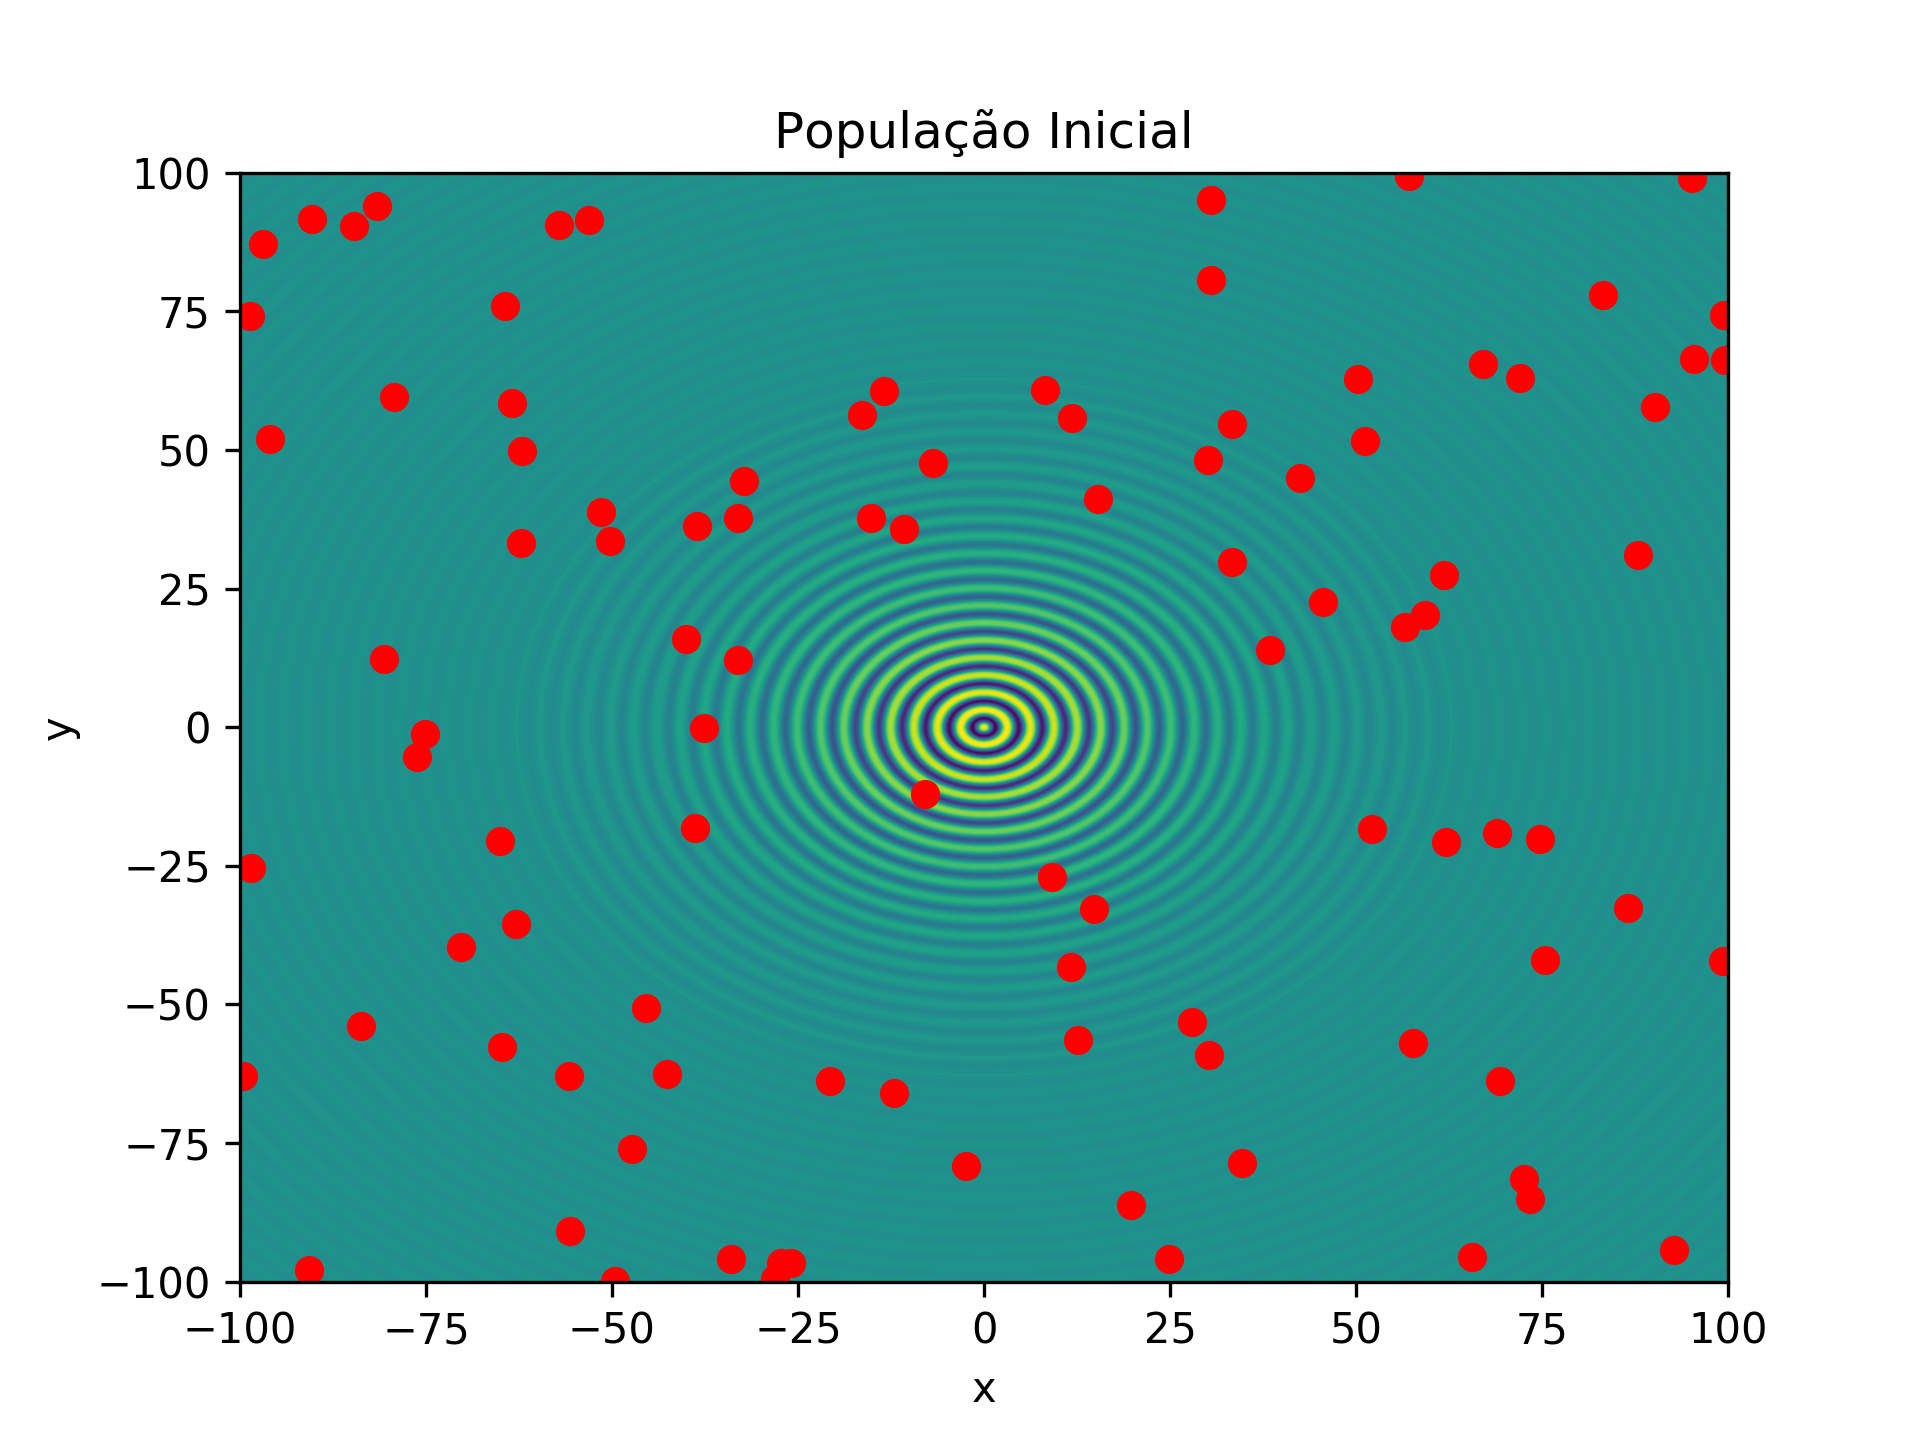
\includegraphics[width=0.9\linewidth]{./imgs/population_gen_0_exp_0.png}
	  \end{subfigure}
	  \begin{subfigure}{.5\textwidth}
		\centering
		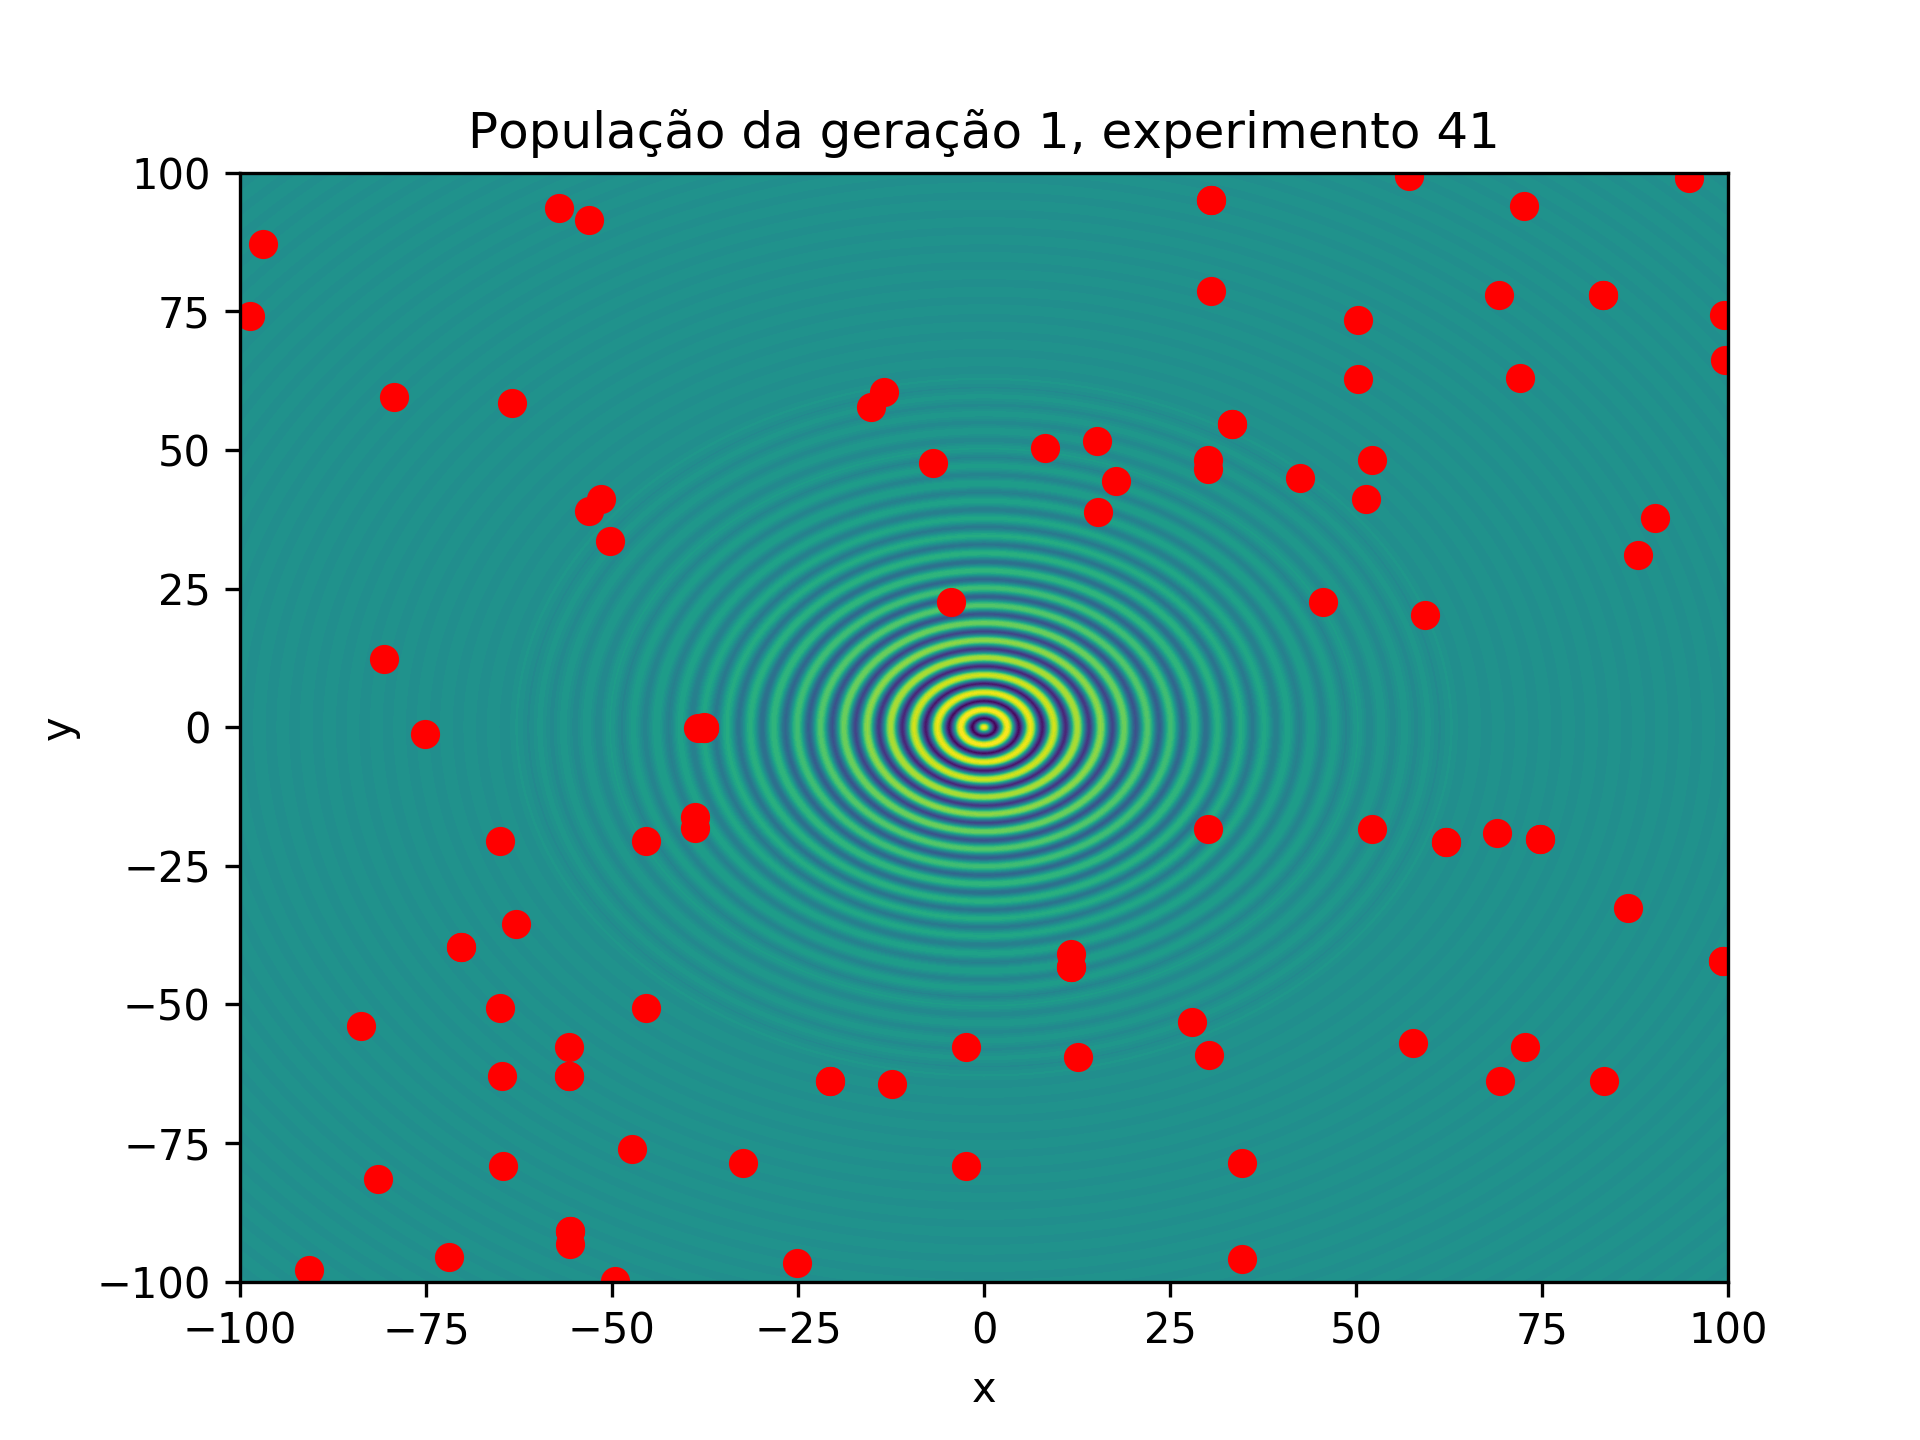
\includegraphics[width=0.9\linewidth]{./imgs/population_gen_0_exp_40.png}
	  \end{subfigure}
	  \begin{subfigure}{.5\textwidth}
		\centering
		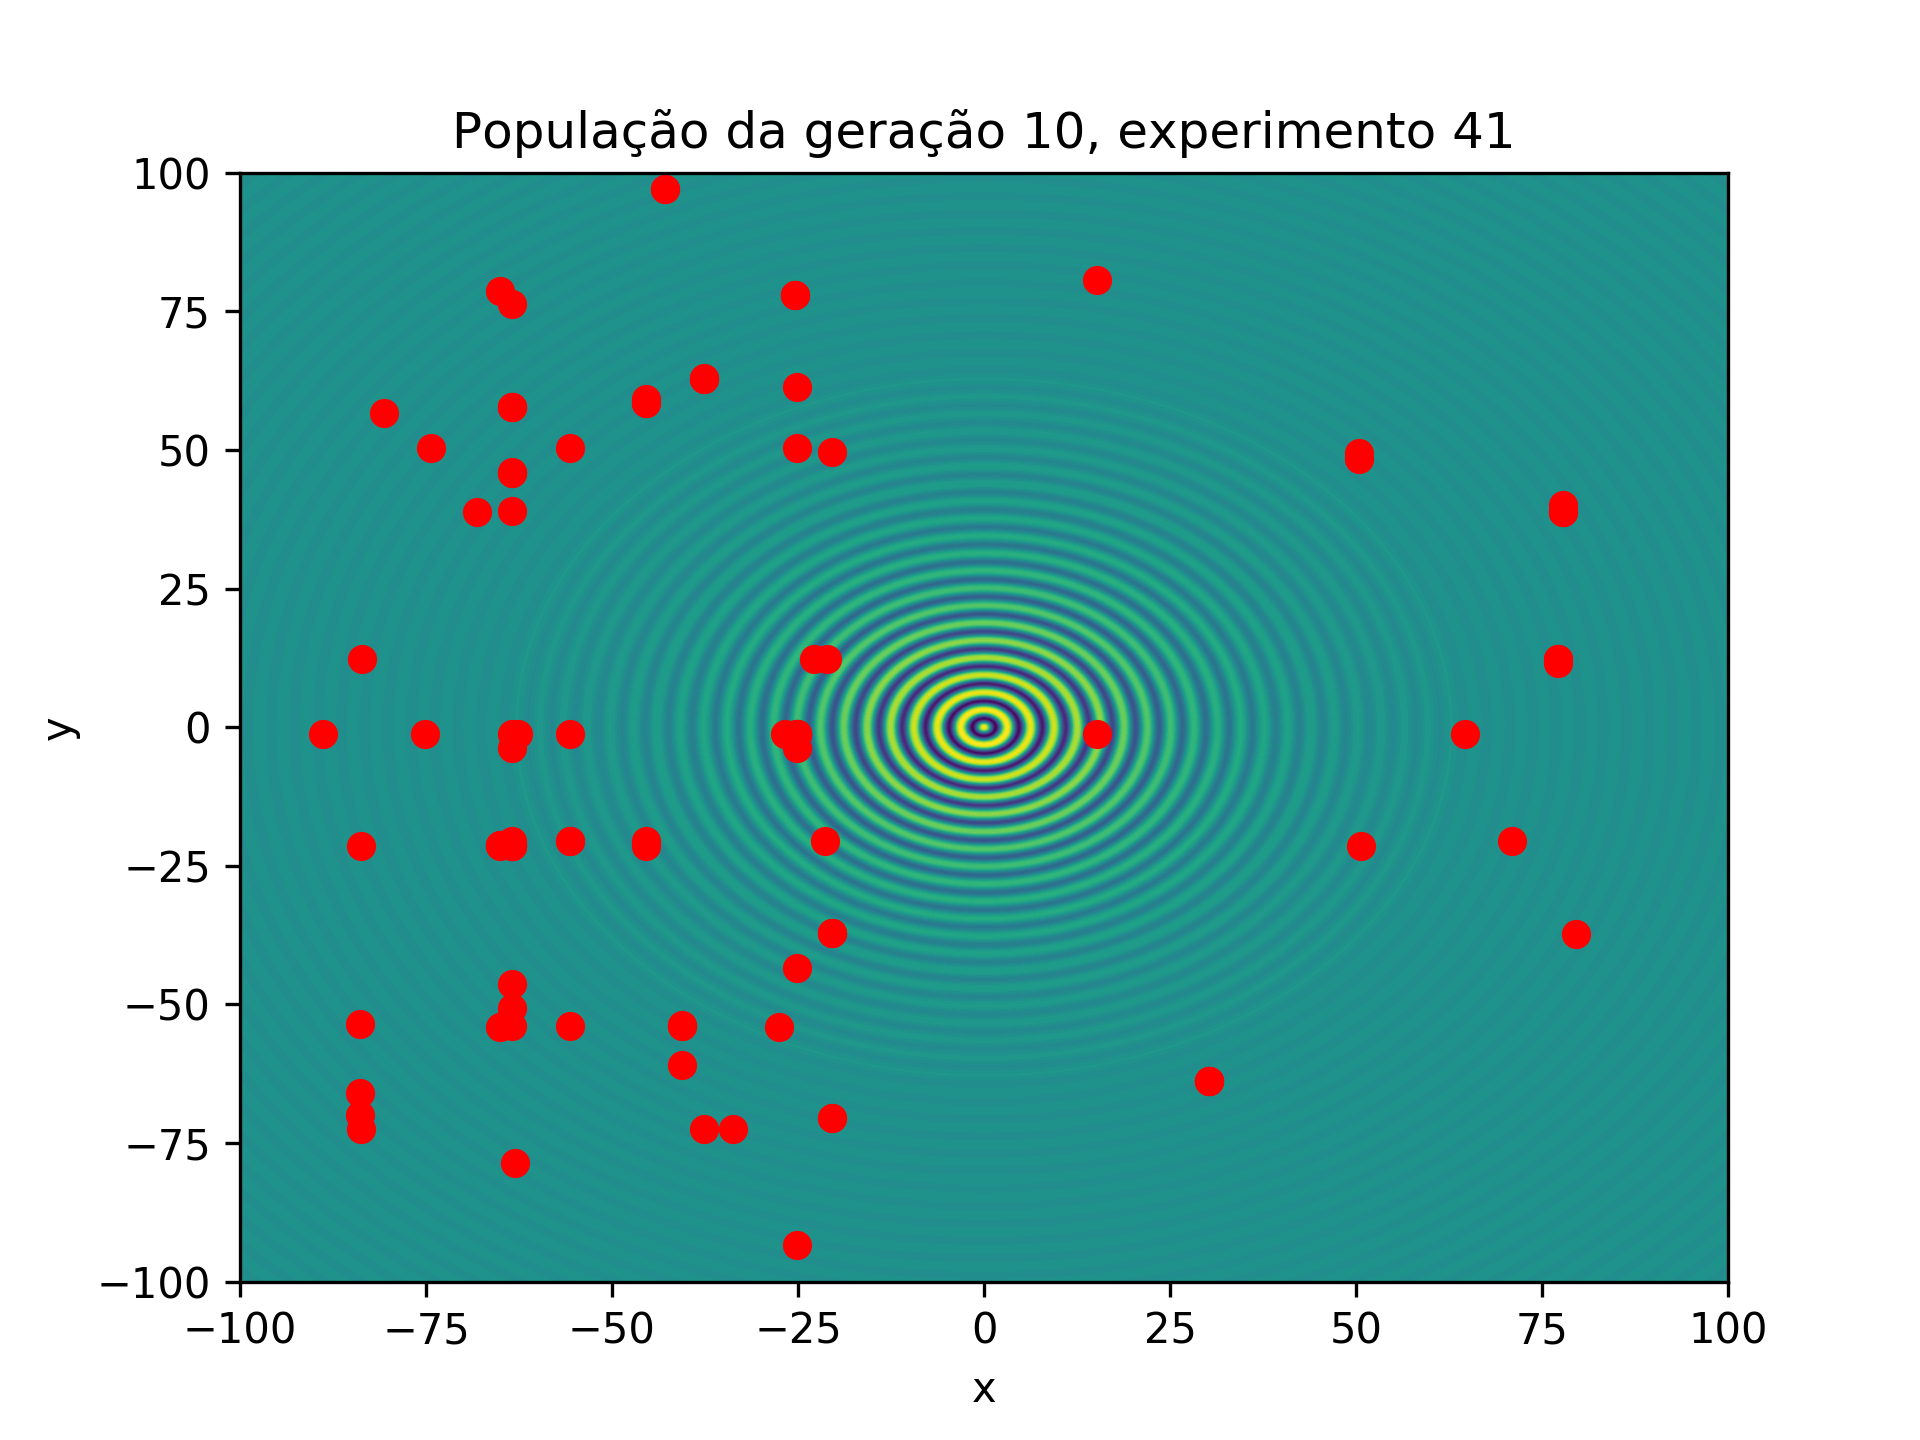
\includegraphics[width=0.9\linewidth]{./imgs/population_gen_9_exp_40.png}
	  \end{subfigure}
	  \begin{subfigure}{.5\textwidth}
		\centering
		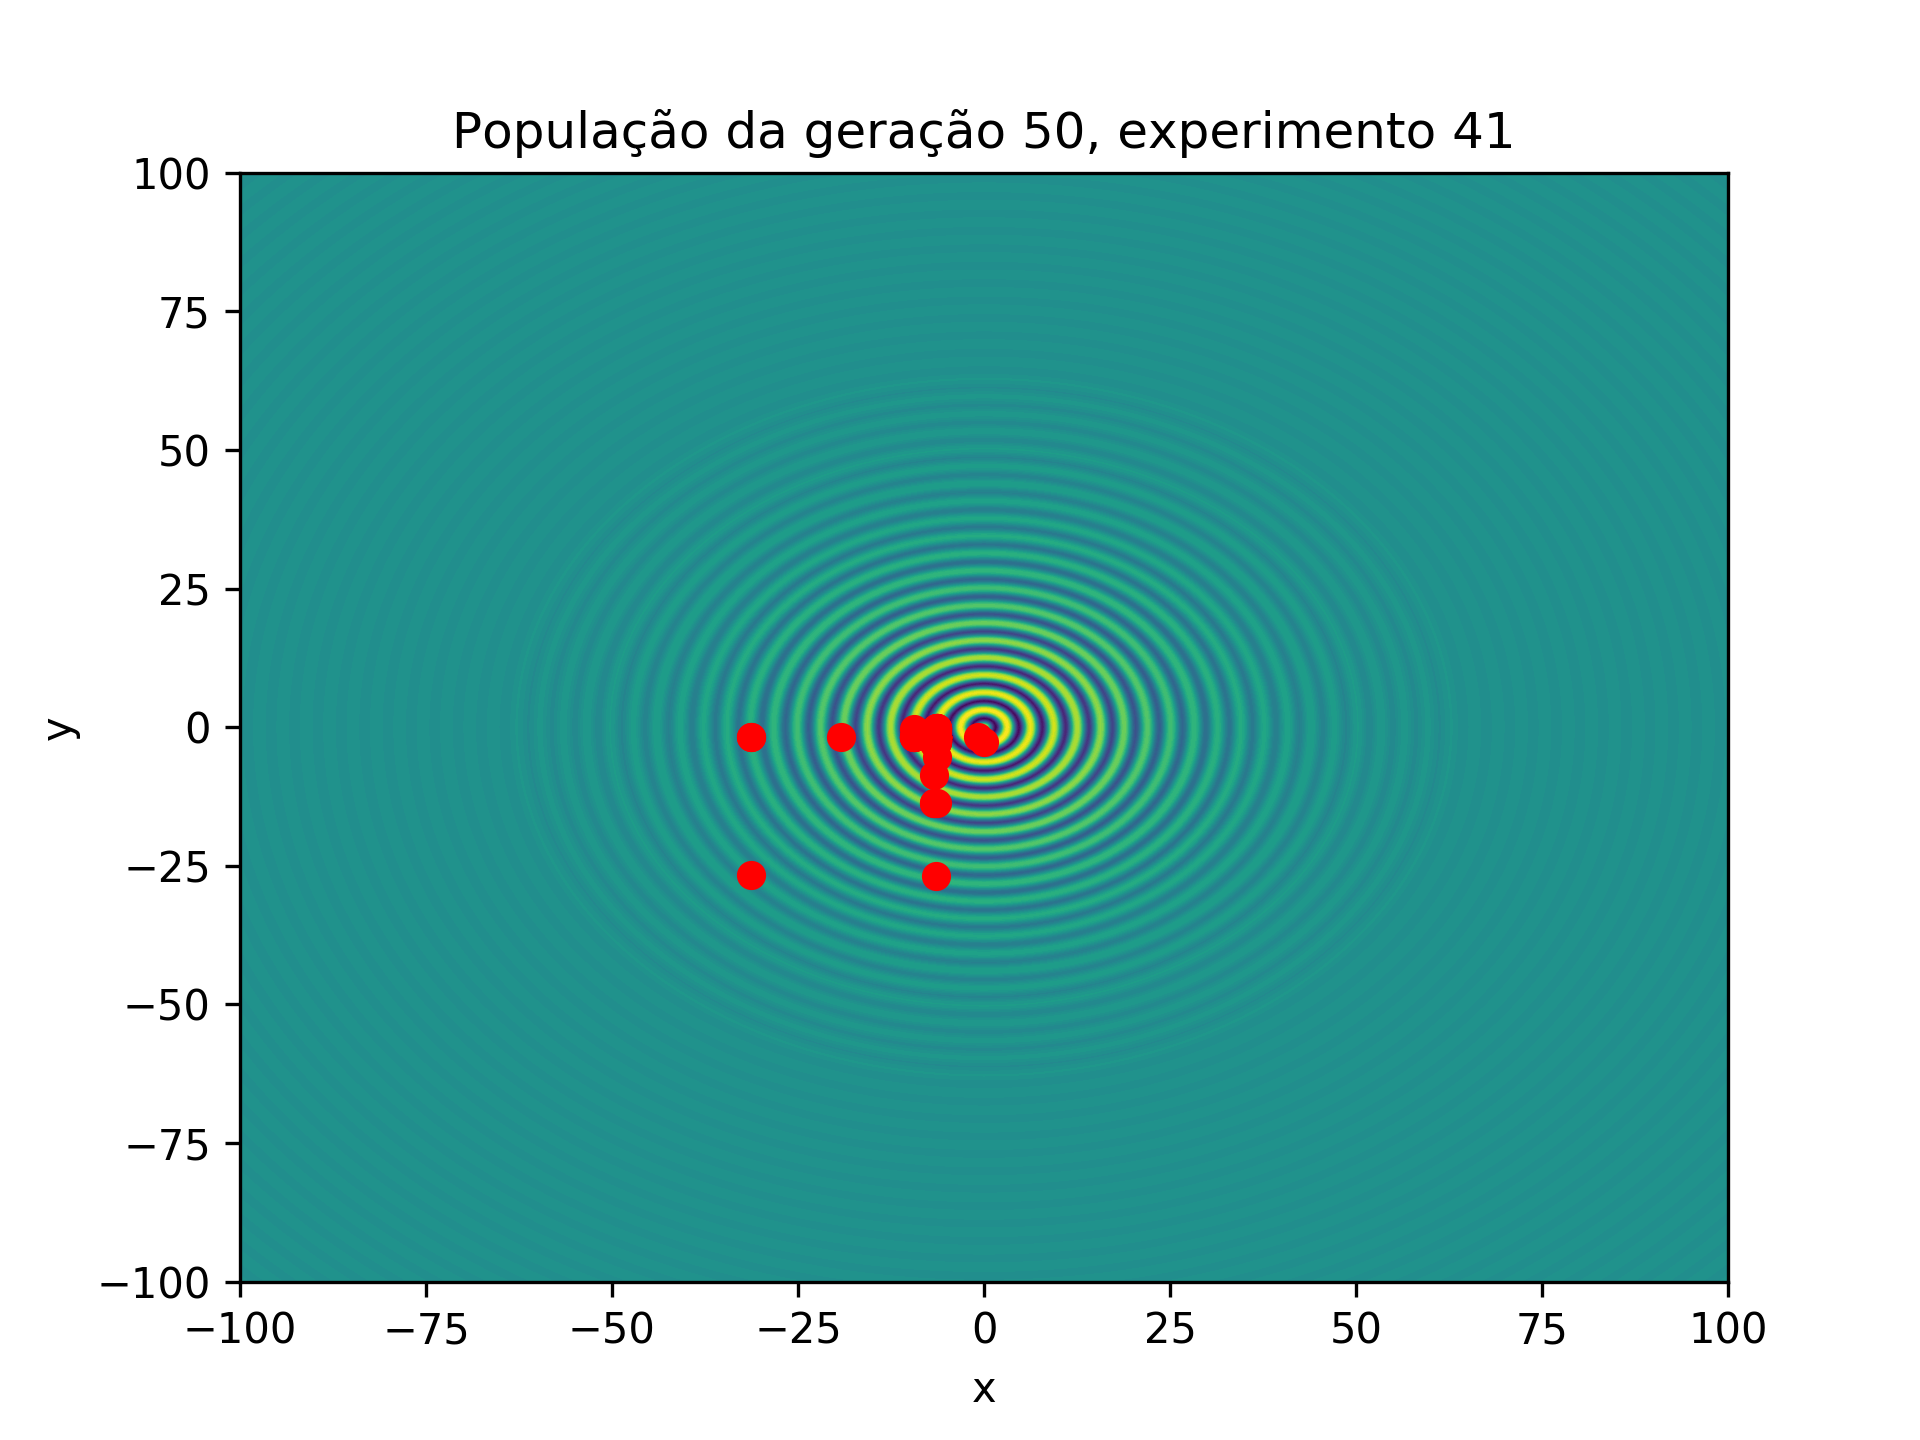
\includegraphics[width=0.9\linewidth]{./imgs/population_gen_49_exp_40.png}
	  \end{subfigure}
	  \begin{subfigure}{.5\textwidth}
		\centering
		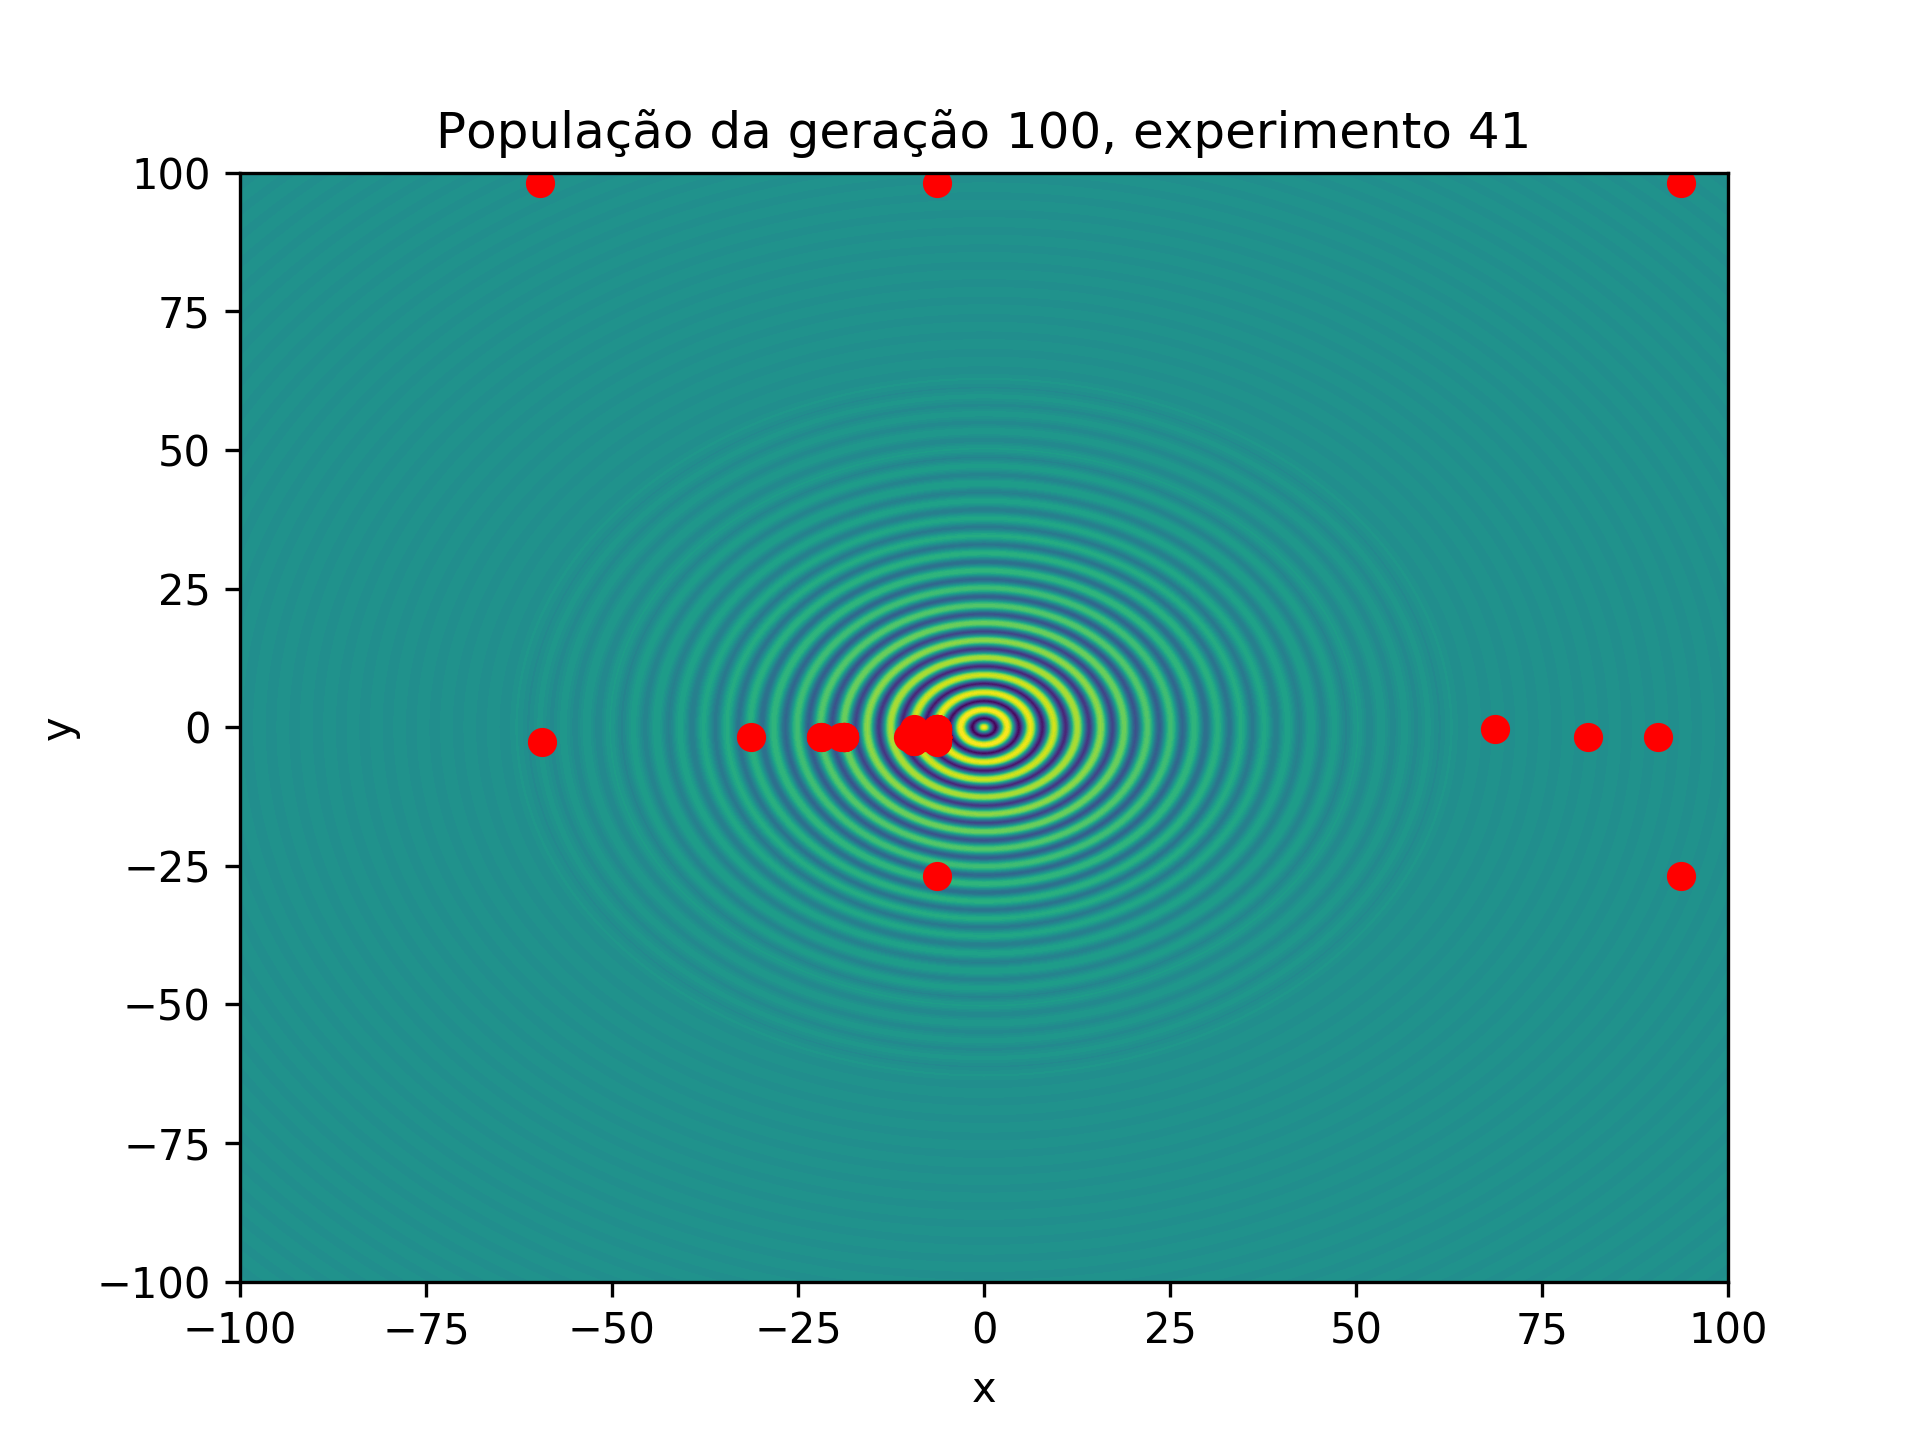
\includegraphics[width=0.88\linewidth]{./imgs/population_gen_99_exp_40.png}
	  \end{subfigure}
	\caption{Populações do experimento 40 nas gerações 1, 10, 50 e 100}
	\end{figure}

\end{document}
